%!TEX root = ../Report.tex

In this chapter, we discuss the results of the experiments and their ramifications. The structure of this chapter mirrors that of the experiments section, so that the first results discussed will be the first experiment detailed in chapter \ref{chapter:experimental_methodology_and_program}. The error bars on the graphs show the standard deviation, and all time measurements are in milliseconds.



\section{Experiment Results}



\subsection{Experiment 1 - Metrics Collection Overhead}

In experiment 1, we investigated our method for collecting metrics, to see if it adds any significant overhead that we must take into account in assessing further experiments. Looking at the following results, particularly the percentage of total runtime, the performance impact of metrics collection is not too severe. Still, detailed metrics were disabled for future experiments.

Of course, in a production system, we would not need any metrics collection.


\begin{figure}[H]
	\centering
	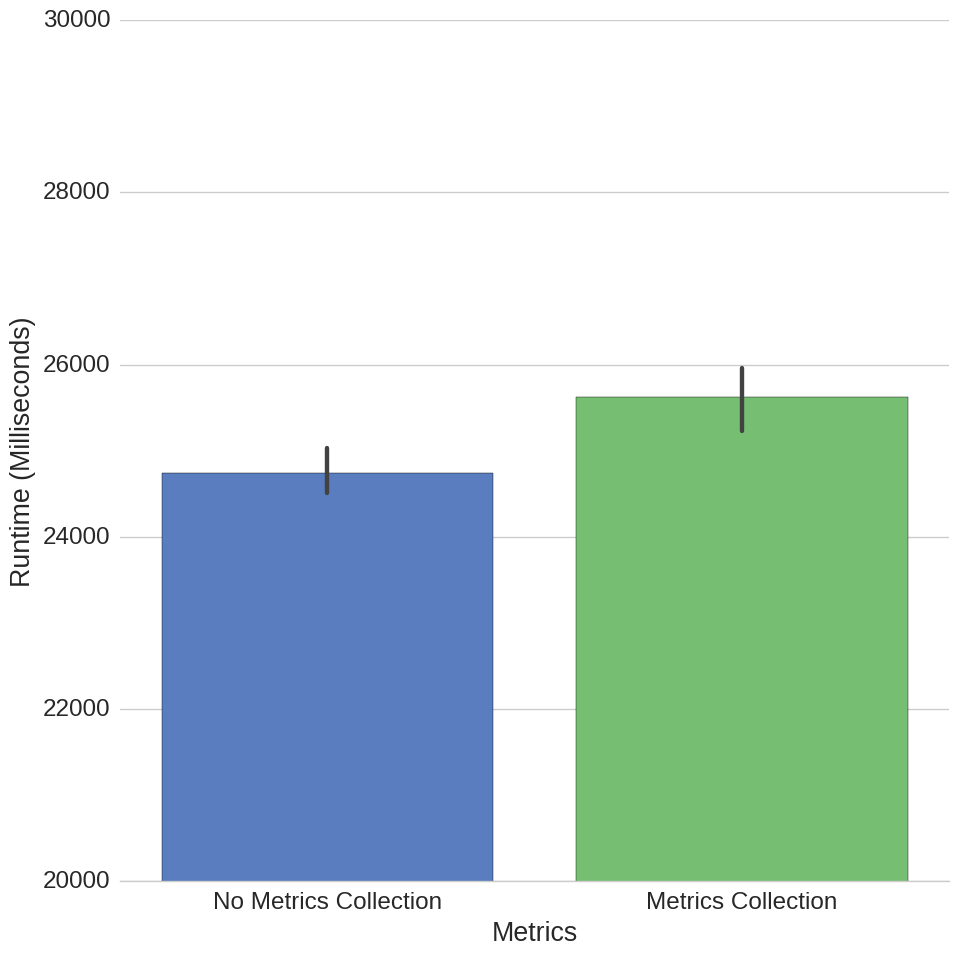
\includegraphics[width=\textwidth]{graphics/experiment1.png}
	\caption{Experiment 1 results}
	\label{fig:results_ex1}
\end{figure}

\begin{table}[H]
\centering
	\begin{tabular}{|c|c|}
		\hline
		Average delay added & 877ms \\
		\hline
		Percentage of total runtime & 3.5\% \\
		\hline
	\end{tabular}
	\caption{Experiment 1 Results Analysis}
	\label{table:results_experiment_1_results_analysis}
\end{table}

%% LaTeX2e file `ex_params/ex1_params.tex'
%% generated by the `filecontents' environment
%% from source `Report' on 2017/03/25.
%%
\begin{table}
\centering
 \begin{tabular}{|c|c|}
  \hline
  Number of tasks & 100,000 \\
  \hline
  Task Grain & 100,000 Repeats \\
  \hline
  Task Grain Distribution & Uniform \\
  \hline
  Number of CPU cores & 4 \\
  \hline
  Number of threads used & 4 \\
  \hline
  Thread pinning & Uniform \\
  \hline
  Schedule & Dynamic Chunks (Chunk Size = 1000) \\
  \hline
 \end{tabular}
\caption{Experiment 1 Parameters}
\iflabela
\label{table:evaluation_ex1_parameters}
\fi
\labelatrue
\end{table}




\subsection{Experiment 2 - Absolute Performance}

In this experiment, the total run times of three implementations are measured. One sequential implementation, a standard modern parallel implementation utilizing OpenMP, and our implementation of map\_array. Our implementation is running with no plasticity for the moment, and with no messaging functionality at all. This is so it is comparable to a standard parallel implementation, since the purpose of this experiment is to test our baseline performance.

Figure \ref{fig:results_ex2} shows us that with a single thread, our performance is similar to a sequential implementation, and as we increase the thread count, our performance scales accordingly. Overall, this shows that our implementation performs on a par with current parallel implementations, providing a good baseline performance. 



\begin{figure}
	\centering
	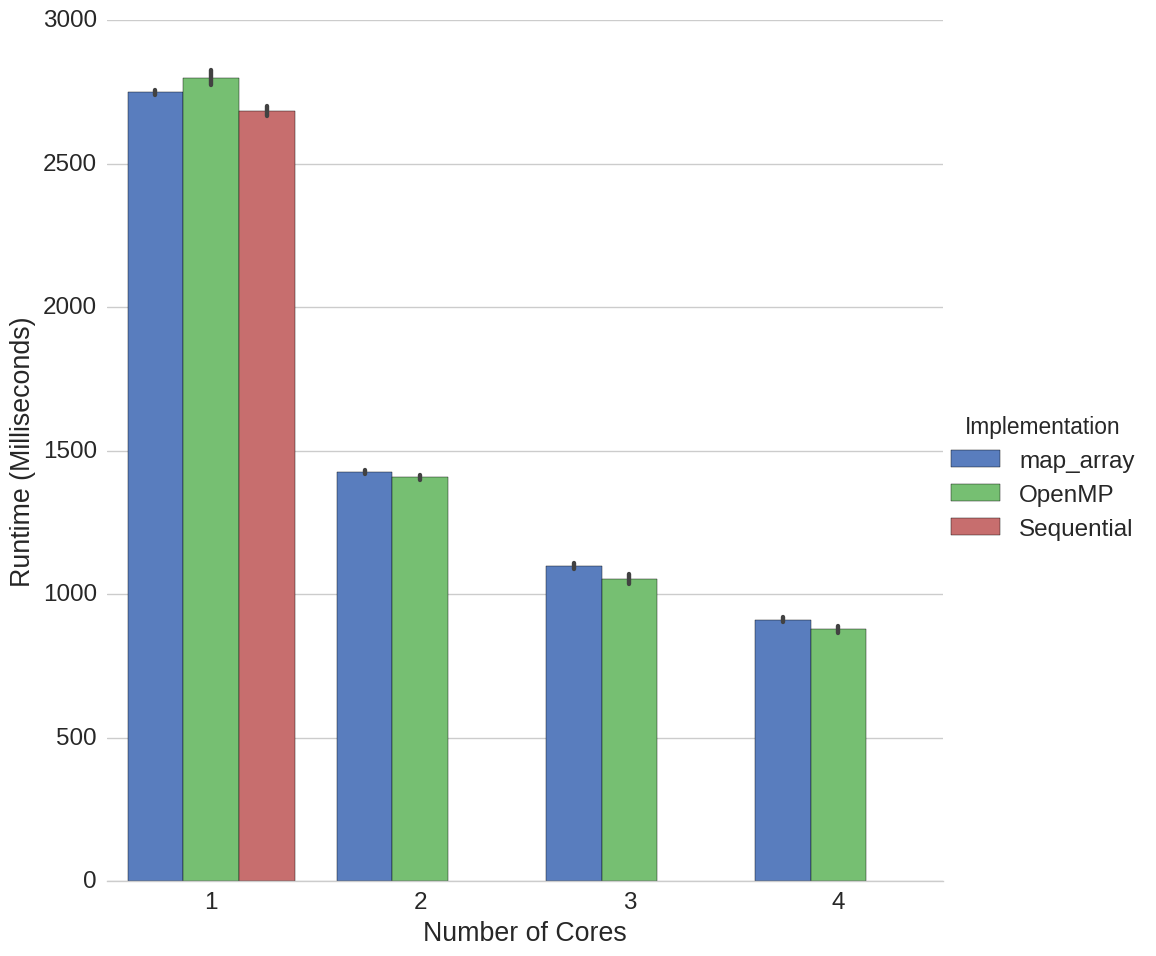
\includegraphics[width=\textwidth]{graphics/experiment2.png}
	\caption{Experiment 2 results}
	\label{fig:results_ex2}
\end{figure}

%% LaTeX2e file `ex_params/ex2_params.tex'
%% generated by the `filecontents' environment
%% from source `Report' on 2017/03/25.
%%
\begin{table}
\centering
 \begin{tabular}{|c|c|c|c|}
  \hline
  Number of tasks & 10,000 \\
  \hline
  Task Grain & 1,000,000 Repeats \\
  \hline
  Task Grain Distribution & Uniform \\
  \hline
  Number of CPU cores & 4 \\
  \hline
  Number of threads used & \specialcell{1, \\ 2, \\ 3, \\ 4} \\
  \hline
  Thread pinning & Uniform \\
  \hline
  Schedule & Static \\
  \hline
 \end{tabular}
\caption{Experiment 2 Parameters}
\iflabelb
\label{table:evaluation_ex2_parameters}
\fi
\labelbtrue
\end{table}




\subsection{Experiment 3 - Plasticity And Contention Aware Scheduling Framework Overhead}

This experiment was designed to assess the amount of overhead added by plasticity and the contention aware scheduling framework. The results are interesting, because we would expect the runtime to only increase with the added overhead, but we have two cases where the runtime decreases. 

With our smallest array size of 1000, we see an increase of 2ms, which is 2.7\% of the total runtime. These results are very close, and within the margin of error. 

Our other results both show a decrease in runtime, again both within the margin of error. Repeat experiments to reduce the variance would help, and running them on a VM may introduce more variance than in a non-virtualized system.

The overall conclusion from this experiment, is that the added overhead is negligible when measuring the total runtime, with a wide selection of array sizes.



\begin{figure}[H]
	\centering
	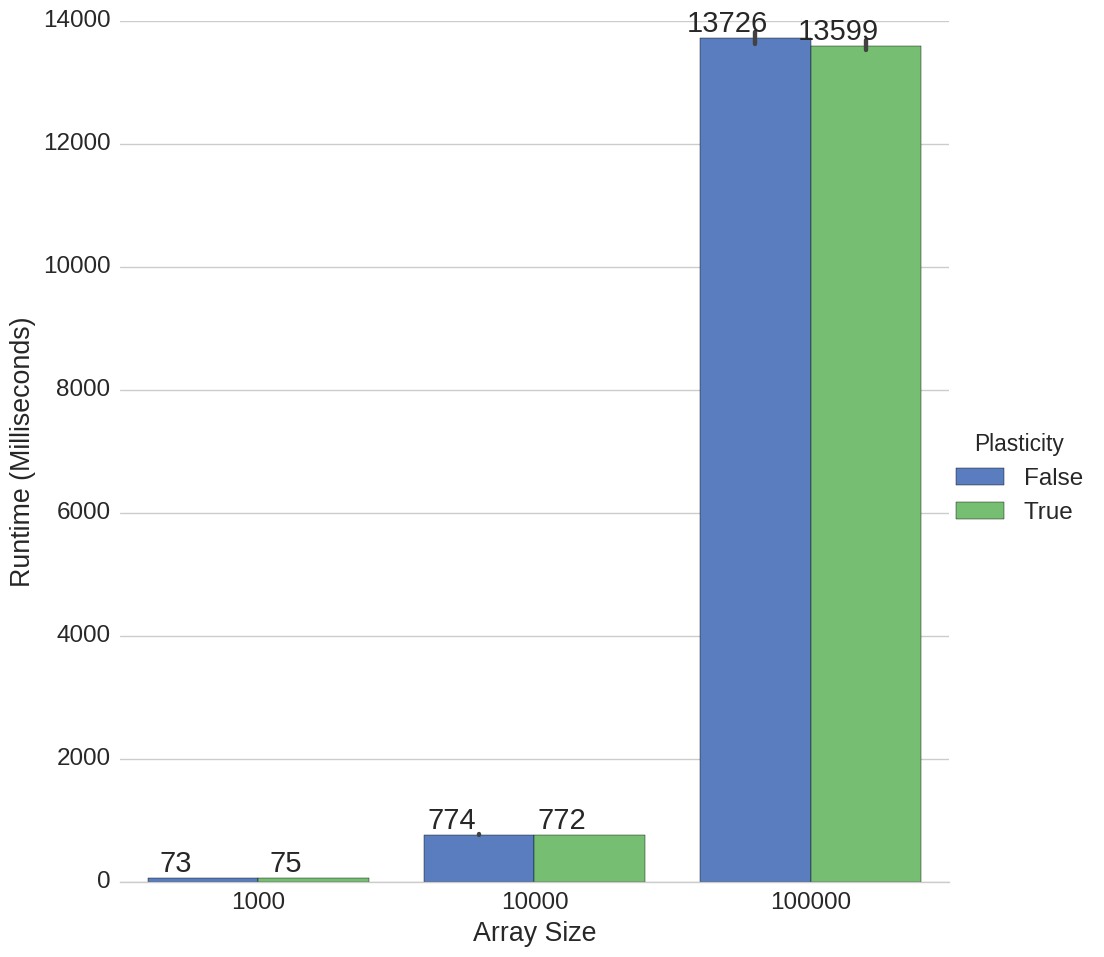
\includegraphics[width=\textwidth]{graphics/experiment3.png}
	\caption{Experiment 3 results}
	\label{fig:results_ex3}
\end{figure}

\begin{table}[H]
\centering
	\begin{tabular}{|c|c|}
		\hline
		Average delay added (Few tasks) & 2ms \\
		\hline
		Percentage of total runtime (Few tasks) & 2.7\% \\
		\hline
		\hline
		Average delay added (Med. tasks) & -2ms \\
		\hline
		Percentage of total runtime (Med tasks) & N/A \\
		\hline
		\hline
		Average delay added (Many tasks) & -127ms \\
		\hline
		Percentage of total runtime (Many tasks) & N/A \\
		\hline
	\end{tabular}
	\caption{Experiment 3 Results Analysis}
	\label{table:results_experiment_3_results_analysis}
\end{table}

%% LaTeX2e file `ex_params/ex3_params.tex'
%% generated by the `filecontents' environment
%% from source `Report' on 2017/03/25.
%%
\begin{table}
\centering
 \begin{tabular}{|c|c|}
  \hline
  Number of tasks & 100,000 10,000 1,000 \\
  \hline
  Task Grain & Medium \\
  \hline
  Task Grain Distribution & Uniform \\
  \hline
  Number of CPU cores & 4 \\
  \hline
  Number of threads used & 4 \\
  \hline
  Thread pinning & Uniform \\
  \hline
  Schedule & Dynamic Chunks \\
  \hline
 \end{tabular}
\caption{Experiment 3 Parameters}
\iflabelc
\label{table:evaluation_ex3_parameters}
\fi
\labelctrue
\end{table}




\subsection{Experiment 4 - Schedule Choice Importance}

This experiment was designed to highlight the importance of choosing the correct schedule, and how we can benefit from runtime plasticity. We have a biased set of tasks, (first quarter of which are large tasks, the rest small,) meaning the static schedule will perform poorly, and the dynamic schedules will fare well.

This is reflected in the results, where we see the dynamic schedules perform almost three times as well as the static schedule. Also included is a case where we start with the static schedule, and then switch to dynamic chunks after five seconds. We see it perform on a par with our dynamic schedules, again greatly improving upon the static schedule.

There is a small difference between our dynamic chunks and dynamic individual schedules. With a chunk size of 1,000, our dynamic individual schedule accesses the bag of tasks 1,000 times as often. Considering that it is implemented in shared memory, it makes sense that this penalty is not large. If retrieving tasks was more costly, it would affect the dynamic individual schedule proportionately more than the dynamic chunks schedule. We also have a variety of task sizes, meaning the time between bag accesses varies. In turn, this means threads are less likely to contend with each other when attempting to obtain the mutex to access the bag.

In our plastic schedule, we change from static to dynamic\_chunks after 5 seconds. In these first 5 seconds, all threads will still have tasks to process, meaning we still have maximum throughput. Since we change to a dynamic schedule before we have any down time, we match the performance of a constant dynamic schedule.



\begin{figure}
	\centering
	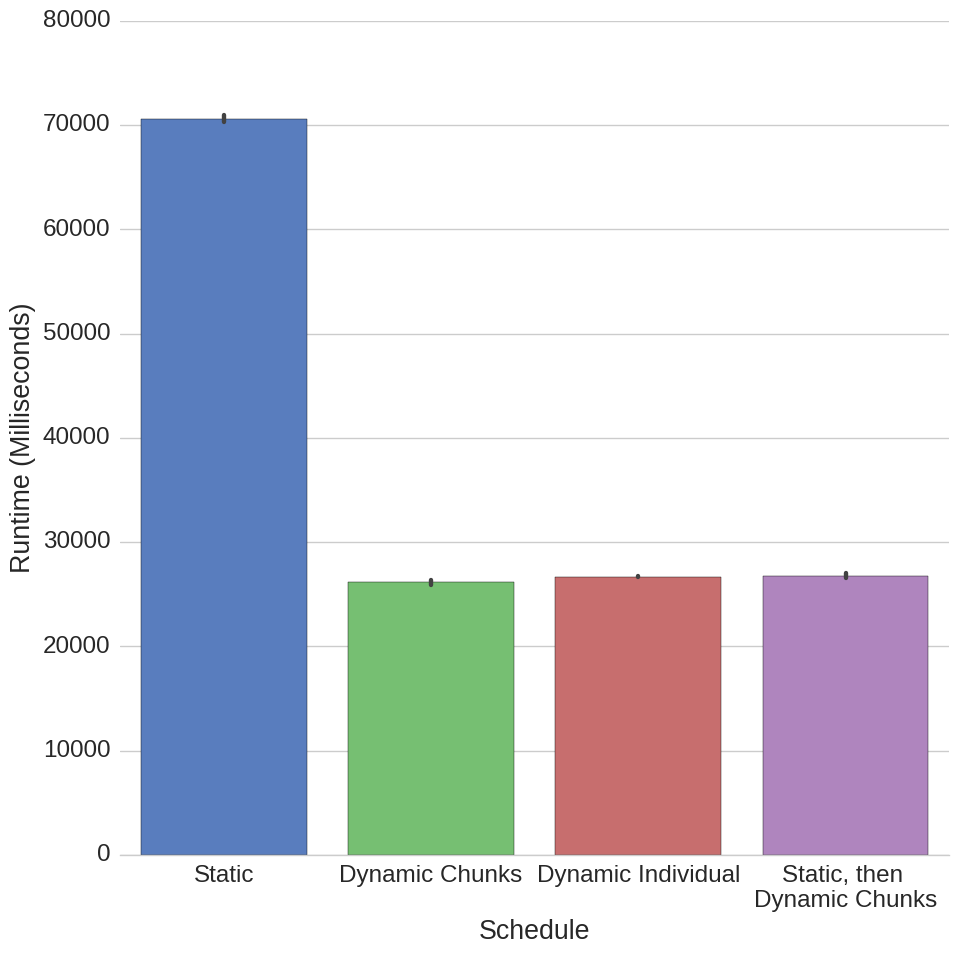
\includegraphics[width=\textwidth]{graphics/experiment4.png}
	\caption{Experiment 4 results}
	\label{fig:results_ex4}
\end{figure}

%% LaTeX2e file `ex_params/ex4_params.tex'
%% generated by the `filecontents' environment
%% from source `Report' on 2017/03/25.
%%
\begin{table}
\centering
 \begin{tabular}{|c|c|}
  \hline
  Number of tasks & 100,000 \\
  \hline
  Task Grain & Large and small \\
  \hline
  Task Grain Distribution & Biased \\
  \hline
  Number of CPU cores & 4 \\
  \hline
  Number of threads used & 4 \\
  \hline
  Thread pinning & Uniform \\
  \hline
  Schedule & \specialcell{Static, \\ Dynamic Chunks (Chunk Size = 1,000), \\ Dynamic Chunks (Chunk Size = 1) \\ Static, then dynamic chunks after 5 seconds} \\
  \hline
 \end{tabular}
\caption{Experiment 4 Parameters}
\iflabeld
\label{table:evaluation_ex4_parameters}
\fi
\labeldtrue
\end{table}




\subsection{Experiment 5 - Absolute Multiprogramming Performance}

The purpose of this experiment is to investigate the absolute performance of our library in a situation with multiple applications. We compare two situations, the first, named anarchy, is where both programs are run with four threads with no plasticity or contention aware scheduling. This is a typical situation for a multiprogramming system. In the second situation, we use plasticity and contention aware scheduling, where we start with four threads in program 1, once program 2 starts we reduce this to two, and assign two threads to program 2. Once program 2 is finished, we switch back to using four threads in program 1.

For a further investigation into the performance of our library, and on a hunch, we also ran the experiment with different message checking intervals. This means that each program's main thread sleeps for Nms in between checks for whether the computation is complete or if it has any messages.

Looking at the results, our library is consistently faster than anarchy, which is a promising sign. We also significantly reduce the variance using our library, possibly due to the reduced thread switching. Comparing the different sleep times, we see that significant improvements can be made, if we tune this variable correctly. Since we are reducing some overhead by making this interval longer, (with the compromise of a slower reaction speed to messages), we could reason that if the library were more sophisticated, and if we thoroughly optimized our code, we may see substantial performance gains.

There is an interesting performance gain going from a 20ms checking interval to a 100ms interval. While unusual, it held for the 50 repeats, so it is not an isolated case. Due to time constraints, this could not be investigated further, but this could be a possibility for the future work in the next year of this MInf project.



\begin{figure}
	\centering
	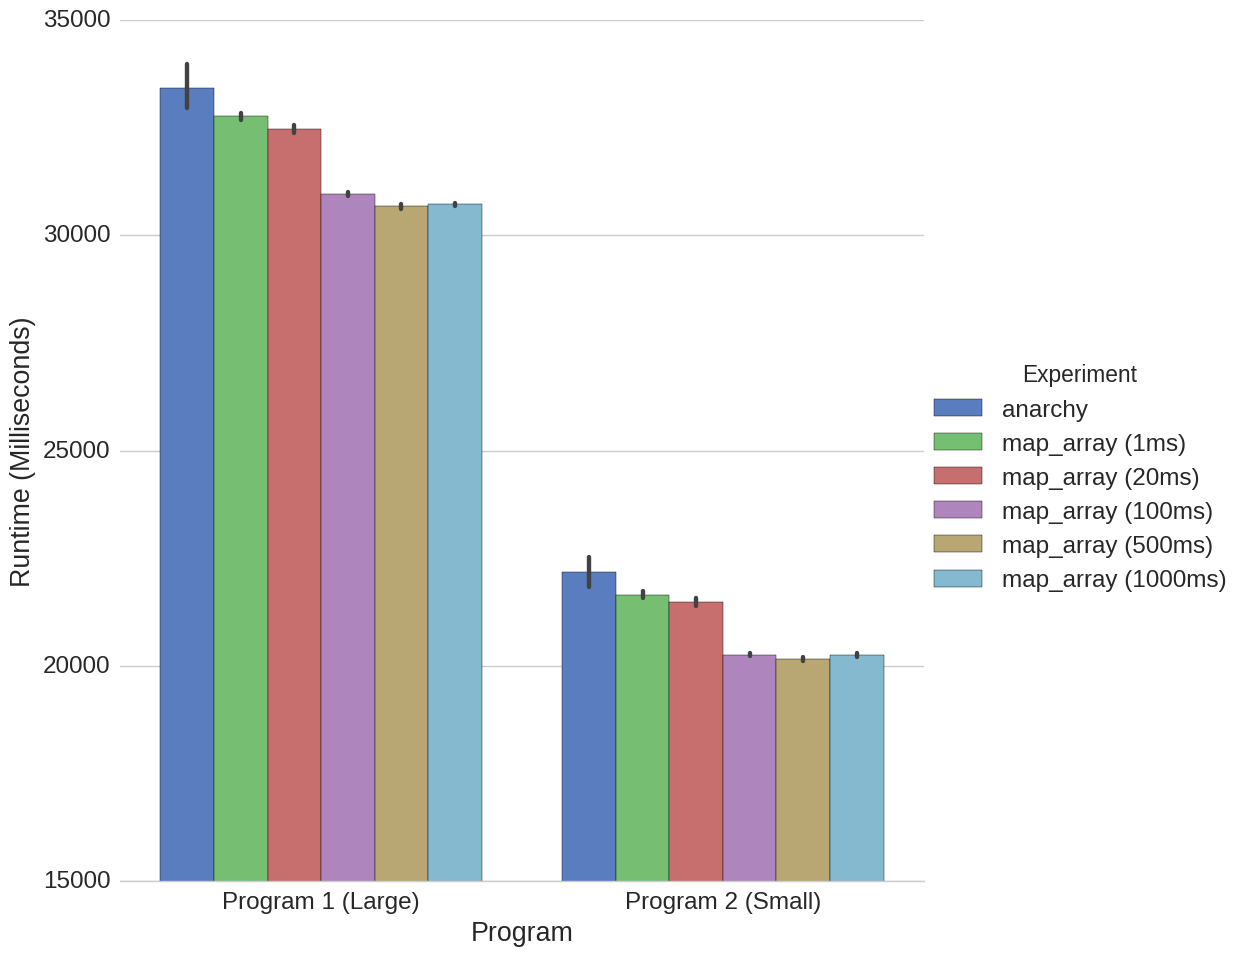
\includegraphics[width=\textwidth]{graphics/experiment5.png}
	\caption{Experiment 5 results}
	\label{fig:results_ex5}
\end{figure}

%% LaTeX2e file `ex_params/ex5_params.tex'
%% generated by the `filecontents' environment
%% from source `Report' on 2017/03/25.
%%
\begin{table}
\centering
 \begin{tabular}{|c|c|}
  \hline
  Program 1 & \\
  \hline
  Number of tasks & 30,000 \\
  \hline
  Task Grain & 10,000,000 Repeats \\
  \hline
  Task Grain Distribution & Uniform \\
  \hline
  Number of CPU cores & 4 \\
  \hline
  Number of threads used & \specialcell{4 \\ 4, then 2, then 4} \\
  \hline
  Thread pinning & \specialcell{Loose, \\ Uniform} \\
  \hline
  Schedule & Dynamic\_individual \\
  \hline
 \end{tabular}

 \begin{tabular}{|c|c|}
  \hline
  Program 2 & \\
  \hline
  Number of tasks & 15,000 \\
  \hline
  Task Grain & 10,000,000 Repeats \\
  \hline
  Task Grain Distribution & Uniform \\
  \hline
  Number of CPU cores & 4 \\
  \hline
  Number of threads used & \specialcell{4 \\ 2} \\
  \hline
  Thread pinning & \specialcell{Loose, \\ Uniform} \\
  \hline
  Schedule & Dynamic\_individual \\
  \hline
 \end{tabular}
\caption{Experiment 5 Parameters}
\iflabele
\label{table:evaluation_ex5_parameters}
\fi
\labeletrue
\end{table}




\section{Conclusion}

In this section, we discuss the implications of each experiment, and what they mean for the future of the project. 

Experiment 1 investigates the overhead added by detailed metrics collection. These metrics were mostly used during development, and as such were disabled for future experiments to minimize their performance impact. 

Experiment 2 establishes a baseline of performance, confirming that we are on a par with current parallel programming approaches. This is a positive result, and confirms that our approach does not concede significant overhead. 

Experiment 3 investigates the overhead involved in contention aware scheduling and plasticity. The results build upon the conclusion of experiment 2, in that we do not add any significant overhead, this time by measuring the overhead of plasticity and contention aware scheduling.

Experiment 4 is a demonstration of the value of choosing the correct schedule, and shows the benefits of plasticity. 

Experiment 5 confirms that we can improve upon our standard implementation with plasticity and contention aware scheduling. We also see reduced variability, both of which are promising results for the early stages of this project. It provides a solid foundation for the next phase in the following year. We also show that we can improve our performance further by optimizing and tuning the code, again providing promising work for the future.

A future system would be useful in any performance orientated application, even when the machine will only be running a single instance, as we can still optimize the implementation to the environment on that machine (as demonstrated in experiment 4.) It would, however, come into its own when we have multiple instances running simultaneously on a machine, a common situation with modern multiprogramming machines.

Overall, the first year of this project has provided a solid foundation for the work to be done next year, and future work for others following the completion of the project.